\chapter{Results}
\usepackage{float})
In the previous chapter, it was explained how the modelling was to be done. In this chapter, the results obtained from the simulation will be evaluated. The evaluation was done by obtaining the results of PHREEQC simulation and processing them into software package like MATLAB to obtain graphical results for clear understanding. 
    As mentioned, the idea was to focus on three main minerals: Aragonite, Calcite and Dolomite. However, when using the results of Dolomite they were interfering with the values and hence were disregarded. A solution with Dolomite is attached in Appendix A.
\newline
\newline
Since the simulation was done for mainly five types of mixture as shown in Table \ref{tablemix}, the result of all these mixtures will be evaluated in brief in the following subsections with their change in regard to temperature, pressure and saturation index at re-injection level.

\begin{table}[h!]
\label{tablemix}
\centering
\caption{Mixture of the fluids with their percentages}
\begin{tabular}{|l|l|l|}
\hline
\textbf{Mix \#} & \textbf{Pure Water (\%)} & \textbf{Brine Fluid (\%)} \\ \hline
\textbf{1}      & 70                       & 30                             \\ \hline
\textbf{2}      & 30                       & 70                             \\ \hline
\textbf{3}      & 50                       & 50                             \\ \hline
\textbf{4}      & 99                       & 1                              \\ \hline
\textbf{5}      & 1                        & 99                            \\ \hline

\end{tabular}
\end{table}

\section{Mixture 1 - 7:3}
In this subsection, the first mixture with 70\% pure water and 30\% brine solution is discussed. 
\begin{figure}[h!]
    \centering
    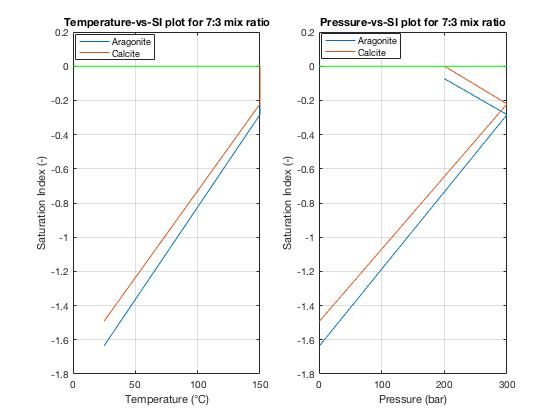
\includegraphics[scale=0.7]{7-3-ratio.jpg}
    \caption{Change in SI with Temperature and Pressure for 7:3 mix }
    \label{fig:7-3}
\end{figure}
 It can be observed in Figure \ref{fig:7-3} that when 70\% of pure water is mixed with 30\% of the brine solution in the reservoir, the saturation index increases as the temperature changes from in-situ to 150 Celsius to the end of the injection well. However, neither calcite nor aragonite have precipitated out since the saturation index is still less than zero. This indicates that the minerals are still dissolved in the mineral. There is a change in the saturation index and hence precipitation of calcite as the pressure decreases from 300 bar to 200 bar when the geothermal fluid starts to move from the injection well to the reservoir and then to the production well. This is one of the reason why production wells are often found to have a higher amount of scaling when compared to the injection well. 
 
 \begin{table}[h!]
\begin{tabular}{|l|l|l|l|l|}
\centering
\label{7-3table}
\caption{SI values for Mix - 1}
\hline
Pressure (bar) & Temperature ( C) & SI$_{Aragonite}$ & SI$_{Calcite}$ & SI$_{Dolomite}$ \\ \hline
1              & 25               & -1.6342       & -1.4904     & -4.4183      \\ \hline
300            & 150              & -0.2833       & -0.2208     & -3.1787      \\ \hline
200            & 150              & -0.0727       & 0.0006      & -2.7522      \\ \hline
\end{tabular}
\end{table}
\section{Mixture 2 - 3:7}
In this subsection, the first mixture with 30\% pure water and 70\% brine solution is discussed. 

\begin{figure}
    \centering
    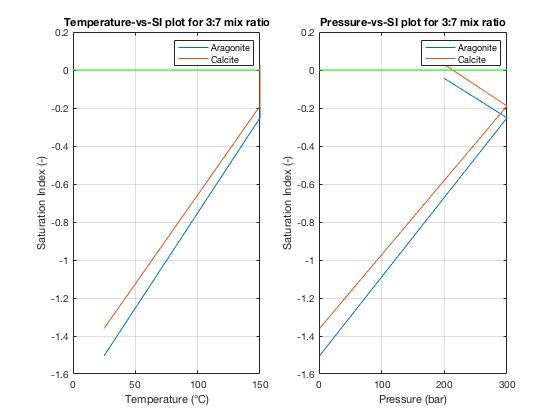
\includegraphics[scale=0.7]{3-7ratio.jpg}
    \caption{Change in SI with Temperature and Pressure for 3:7 mix }
    \label{fig:3-7}
\end{figure}

\section{Mixture 3 - 5:5}
In this subsection, the first mixture with 50\% pure water and 50\% brine solution is discussed. 

\begin{figure}
    \centering
    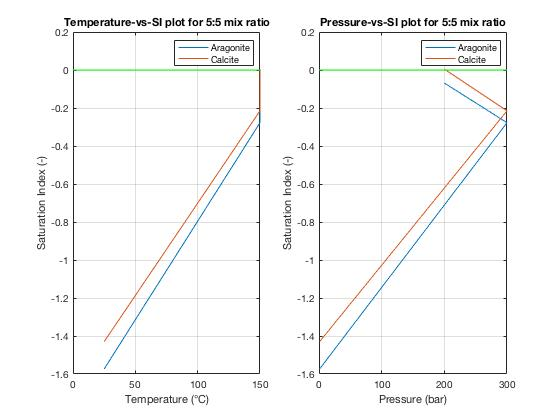
\includegraphics[scale=0.7]{5-5ratio.jpg}
    \caption{Change in SI with Temperature and Pressure for 5:5 mix }
    \label{fig:5-5}
\end{figure}



\section{Mixture 4 - 9.9:0.1}
In this subsection, the first mixture with 99\% pure water and 1\% brine solution is discussed. 


\begin{figure}
    \centering
    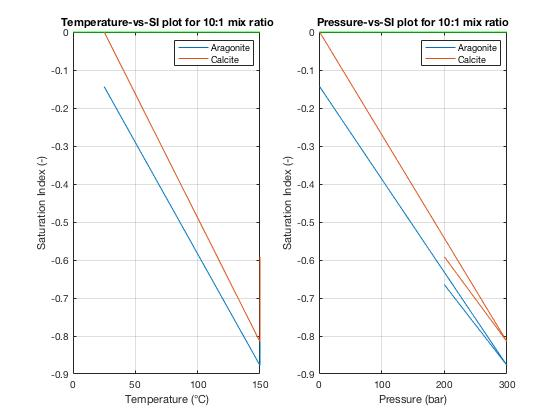
\includegraphics[scale=0.7]{10-1ratio.jpg}
    \caption{Change in SI with Temperature and Pressure for 10:1 mix }
    \label{fig:10-1}
\end{figure}

\section{Mixture 5 - 0.1:99}
In this subsection, the first mixture with 1\% pure water and 99\% brine solution is discussed. 
\begin{figure}
    \centering
    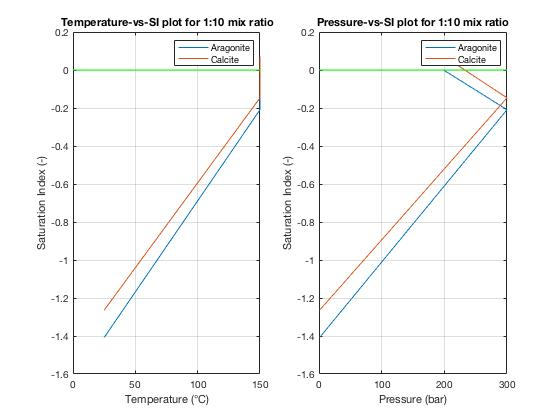
\includegraphics[scale=0.7]{1-10ratio.jpg}
    \caption{Change in SI with Temperature and Pressure for 1:10 mix }
    \label{fig:1-10}
\end{figure}